% !TeX program = pdflatex
% Frontiers of Computer Science submission --- generated from recover-or-abstain-fcs.md
% by submission/fcs/md2fcs_tex.py. Edit the Markdown, not this file.
\documentclass[10pt]{article}
\usepackage[margin=2.2cm]{geometry}
\usepackage{booktabs}
\usepackage{graphicx}
\usepackage{amsmath}
\usepackage{amssymb}
\usepackage{url}

\title{Recover or Abstain: Replay-Verified Recovery for Tool-Calling Agents}

% + marks the corresponding author
\author{Tongsen Wang}





\begin{document}
\maketitle

\begin{abstract}
A tool-calling agent that ``looks fixed'' has not necessarily been fixed in a way anyone can prove. An unverified patch may introduce an irreversible side effect that no one observes. We present RACER (Risk-Aware Counterfactual Execution and Recovery), which recasts recovery as an \emph{auditable assertion} rather than an observed coincidence: a recovery claim is admitted only when the candidate patch completes a strict prefix--patch--suffix counterfactual replay in an isolated, fault-free session initialized from the source seed, and carries a recomputable identity receipt; when the replay predicts an irreversible side effect or a failure, the policy \textbf{abstains} and the patch is never committed. We build a paired benchmark over three semantic domains (flight, hotel, shop), 14 baselines, and two LLM actors (GLM-5.3-Flash as the primary analysis, DeepSeek-V4-Flash as an independent replication). Across 800 episodes and 11,200 records, every record passed a fail-closed admission audit with zero exclusions; the harmful-commit evidence rests on the 1,960 irreversible-track records; the 9,240 main-track records measure recovery and domain generality. On seven pre-registered irreversible-side-effect scenarios that combine four misleading-evidence modes with three trigger faults, non-verifying baselines commit harmful repairs in 510/560 (GLM) and 466/560 (DeepSeek) cases and the no-verification ablation in 70/70 and 64/70, whereas RACER's replay veto converts every such case into harmless abstention (0/140 harmful in both models). The harm-rate difference and veto accuracy are both Holm-significant in both models ($p = 1\times10^{-4}$) with 7/7 scenarios directionally consistent, which triggers the pre-registered cross-model pooled analysis. An independent oracle that recomputes harm labels without reading any replay output reproduces every label, and veto accuracy reaches 70/70 (GLM) and 64/70 (DeepSeek). Main-track recovery is 100\%/100\%/75--78\% across the three domains. We also report negative results: no significant difference from the verification-preserving ablation, and self-healing of injected drop/replace faults. These findings inform the design of fault-injection benchmarks.
\end{abstract}

\section{Introduction}

Automatic recovery in production agents faces a structural tension: \textbf{the repair action is itself risky}. Retrying a non-idempotent operation may charge a customer twice; substituting an argument may violate a task constraint; continuing with insufficient evidence can amplify a local error into a global failure. A line of work on agent failure diagnosis---AgentDebug \cite{ref1}, Who\&When \cite{ref2}, AgentFail \cite{ref3}, and AgenTracer \cite{ref4}---answers \emph{where} the failure is, and CausalFlow \cite{ref5} brings counterfactual repair into attribution. Yet the existing evaluation pipeline omits one step: \textbf{how a recovery claim is to be proven}. When a baseline reports ``repair succeeded'', a reviewer or a deployer has no recomputable evidence chain with which to distinguish three very different situations: the repair genuinely happened; the repair happened to be harmless but was never verified; or the repair introduced a side effect that went unobserved.

Our central claim is that \textbf{recovery must be a provable assertion, not an observed coincidence}. We operationalize this claim in four layers:

\begin{enumerate}

  \item \textbf{Public-evidence diagnosis.} Root-cause candidates are derived only from evidence visible in the trajectory (requested-vs-effective action mismatch, error strings, constraint violations); ground truth is physically isolated from the agent.

  \item \textbf{Risk--utility gating.} Candidates are ranked by utility and turned into a patch; when confidence is insufficient or no patch exists, the policy explicitly abstains---abstention is a first-class action.

  \item \textbf{Isolated counterfactual replay.} The patch is replayed in a clean session initialized from the source seed with an empty fault schedule; the receipt must pass an independent recomputation of a 7-field identity contract. When the replay predicts a side effect or a failure, the system \textbf{vetoes the commit} (replay veto).

  \item \textbf{Fail-closed admission.} Records without a provenance anchor, without a replay receipt, without a refund-ledger witness, or containing ground-truth leakage are refused entry to the main table.

\end{enumerate}

\textbf{Contributions.}

\begin{itemize}

  \item \textbf{C1 (Formalization).} A strict semantics for \emph{replay-verified recovery}: a recovery succeeds if and only if the isolated replay evaluates successfully, has no side effect, and carries a receipt satisfying the strict-replay contract; together with the decision semantics of the \textbf{replay veto} (predict harm $\to$ abstain, do not commit). Under this semantics we systematically compare 14 baselines.

  \item \textbf{C2 (Method).} The RACER framework and its accompanying family of fail-closed admission auditors (record-level G1--G7, evaluator-level G0/G8), which turn a recovery claim from a narrative into a machine-checkable credential.

  \item \textbf{C3 (Benchmark).} A paired, pre-registered benchmark with two tracks: a retryable-fault track (3 domains $\times$ 11 cells $\times$ 10 seeds) and an irreversible-side-effect track (7 independent scenarios $\times$ 3 domains $\times$ 10 seeds, with four misleading-evidence modes---omission, price corruption at the budget boundary, stock falsification, and stale quote---crossed with three trigger faults---force\_error, rate\_limit, wrong\_tool---such that ``repair'' means ``commit an irreversible suboptimal decision''). Across 14 baselines and two models the study yields 11,200 records, with protocols, matrices, model resources, and baseline registries frozen and hash-anchored. A negative G4 result on an adaptation of $\tau^{2}$-airline (native refund operations are non-idempotent and expose no ledger witness) motivates the environment design.

  \item \textbf{C4 (Findings).} (i) A 2$\times$2 ablation (gating $\times$ verification) shows that replay verification is a behaviorally necessary component for preventing harmful commits: every policy without verification commits harmful repairs at scale in both models---including the oracle root-cause baseline, i.e. \emph{correct diagnosis does not imply safe repair}---whereas every policy with verification yields only harmless abstention; harm labels recomputed by an oracle that never reads replay output reproduce every row. (ii) Both hypotheses H-E3a and H-E3b are Holm-significant in both models ($p = 1\times10^{-4}$) with 7/7 scenarios directionally consistent, satisfying the pre-registered condition for cross-model pooling. (iii) The three-domain main table exposes a recovery-rate gap under the \texttt{in\_stock} hard gate of the shop domain (75--78\% vs 100\%): the framework behaves consistently across domains, and the gap reflects environmental reachability rather than framework failure. (iv) Injected drop/replace faults are self-healed by the LLM actor's natural re-issuing behavior---fault injection must interact with the agent policy to produce a persistent failure. (v) A null result: no significant difference from the verification-preserving ablation, so the contribution of risk gating lies in declaration discipline rather than in outcome gain.

\end{itemize}

\section{Related Work}

\textbf{Failure diagnosis and attribution.} AgentDebug \cite{ref1} learns failure modes from targeted feedback; Who\&When \cite{ref2} studies automated failure attribution in multi-agent systems; AgentFail \cite{ref3} builds a dataset and taxonomy of the failure lifecycle in platform-orchestrated agentic workflows; and AgenTracer \cite{ref4} distinguishes and localizes the failure-inducing agents in LLM systems. This line continuously refines \emph{where} the root cause is, but its evaluation stops at attribution accuracy: the recovery decision---whether to act, and how to prove that acting was correct---is left to the deployer. RACER is orthogonal and complementary: it takes diagnosis output as an input and studies the trustworthiness of the subsequent repair action. A finding from our irreversible-side-effect track underscores the separation: even with perfect root-cause diagnosis (the \texttt{oracle\_root\_cause} baseline), the repair action is still harmful in every case on irreversible faults---diagnostic correctness and repair safety are two independent dimensions.

\textbf{Counterfactual repair and side-effect safety.} CausalFlow \cite{ref5} proposes counterfactual repair on top of causal attribution and is the closest work to ours, but its repair evaluation does not require a recomputable replay receipt, treats side effects via post-hoc annotation rather than audit-based admission, and has no ``predict harm, therefore do not commit'' veto semantics. $\tau$-bench \cite{ref6} provides a tool--agent--user interaction domain emphasizing domain realism and user simulation, but offers no mechanism for proving a recovery claim; our adaptation experiment on its airline domain (\S6.8) shows that native refund tools are non-idempotent and expose no public ledger witness, so a side-effect claim cannot satisfy fail-closed auditing---this is the direct motivation for the auditable environment and refund-ledger semantics we build. AgentDojo \cite{ref7} evaluates injection-attack defenses in dynamic environments; its injections serve security rather than recovery trustworthiness. The \texttt{tamper\_result} fault in our E3 track (corrupting tool-response payloads) is mechanistically adjacent to prompt injection but acts on recovery evaluation rather than on the attack surface.

\textbf{Methodology of agent evaluation.} Recent benchmark work emphasizes reproducibility and contamination resistance (fixed task sets, seeds, frozen metrics), but ``results are reproducible'' and ``claims are auditable'' are two different levels: the former guarantees that a re-run agrees, while the latter guarantees that every conclusion in a single run is backed by a machine-checkable evidence chain. RACER's paired identity (6-tuple), trial expansion, deduplication proof, and fail-closed admission audit (G0--G8) belong to the latter level. The pre-registration discipline---freeze a protocol before execution, anchor any deviation in a post-hoc reconciliation appendix, and submit artifacts to an independent second auditor---brings practices from empirical software engineering \cite{ref8,ref9} into agent benchmarking; its concrete effect in our project (the second auditor did in fact catch an overstated narrative and force a correction) is reported in \S7.

\textbf{LLM agents and their reliability.} A substantial body of work studies LLM agents as a system paradigm. The agentic loop is explored through reasoning-and-acting \cite{ref10}, self-reflection \cite{ref11} and self-refinement \cite{ref12}; tool use is studied from self-supervised API learning \cite{ref13} to large-scale mastery of real-world APIs \cite{ref14}; benchmarks for agentic behavior range from interactive task suites \cite{ref15,ref16,ref17,ref18} to domain-realistic tool--agent--user interaction \cite{ref6}; and surveys offer broad taxonomies of autonomous agents \cite{ref19,ref20,ref21}. The paradigm also builds on earlier reasoning work---chain-of-thought prompting \cite{ref22}, search over intermediate thoughts \cite{ref23} and multi-agent conversation frameworks \cite{ref24}---as well as on connectors that bind models to large collections of real-world APIs \cite{ref25}. Our work is complementary: rather than proposing a new reasoning loop or a new task suite, we ask what it takes to \emph{prove} that a recovery step was safe, and we show that the answer changes the measured behavior of otherwise comparable strategies.

\textbf{Safety filters and abstention.} The veto has close relatives outside agent recovery. Safety shielding wraps a learning agent with a reactive system that suppresses actions violating a specification, an idea introduced for safe reinforcement learning \cite{ref26}; like a shield, the replay veto is a \emph{pre-commitment} filter whose power comes from judging an action before it takes effect. Selective prediction, or the reject option, formalizes the complementary decision to decline an answer when confidence is insufficient \cite{ref27}; abstention is likewise a first-class action here. The distinguishing element is the evidence standard. A shield enforces a specification supplied a priori, whereas RACER's veto is justified by a recomputed counterfactual execution of that specific patch, and it is the replay receipt---not a hand-written specification---that the admission audit checks.

\section{Problem Formulation}

Let a trajectory be $\tau = (a_0, o_0, \ldots, a_{T-1}, o_{T-1})$, where each action carries a tool name and arguments. The environment injects a fault $f \in \{\text{replace\_action}, \text{force\_error}, \text{rate\_limit}, \text{wrong\_tool}, \text{drop\_action}, \text{tamper\_result}\}$ at a scheduled step; the public trajectory never reveals ground truth. A diagnoser emits a candidate set $D(\tau) = \{(c_i, s_i, p_i, e_i)\}$ of (root cause, step, confidence, evidence) derived only from public evidence. A recovery policy $\pi$ selects $d \in \{\text{retry}, \text{replace\_argument}, \text{ask\_clarification}, \textbf{abstain}\}$ and may generate a patch $\delta$ that substitutes the action at some step.

\textbf{Definition 1 (Replay-verified recovery).} A recovery claim for a patch $\delta$ is \emph{admitted} if and only if there exists an isolated session replay $E(\tau_{\text{cf}})$ that is initialized from the source seed, runs with an empty fault schedule, executes the prefix--$\delta$--suffix sequence, and satisfies (i) $E(\tau_{\text{cf}}).\text{success} = \text{true}$; (ii) $E(\tau_{\text{cf}}).\text{side\_effect} = \text{false}$; and (iii) the replay receipt $r$ satisfies the strict replay contract---seven identity fields recomputed from the source environment contract (contract version, episode, source run, source environment fingerprint, initial-state fingerprint, fault-schedule fingerprint, replay run number) match one by one. A claim failing any of these conditions \textbf{must not be declared a recovery}; the policy may look identical at the behavioral level while its \emph{declaration eligibility} is entirely different.

\textbf{Definition 2 (Replay veto).} If a policy carries a verification layer (\texttt{use\_counterfactual = true}, not \texttt{skip\_counterfactual}), the patch $\delta$ is first evaluated by the isolated replay of Definition 1. When $E(\tau_{\text{cf}}).\text{side\_effect} = \text{true}$ or $E(\tau_{\text{cf}}).\text{success} \neq \text{true}$, the decision is changed to abstain (reasoning recorded as \texttt{replay\_veto\_side\_effect} / \texttt{replay\_veto\_not\_success}) and $\delta$ is \textbf{not committed} to the source environment. A vetoed row is recorded as a harmless abstention: recovery 0, harm 0---``predicted harmful and therefore not committed''.

\textbf{Definition 3 (Paired identity).} Each source episode is uniquely identified by the 6-tuple ($\text{episode\_id}$, $\text{source\_run\_id}$, $\text{task\_id}$, $\text{canonical\_json}(\text{env\_seed})$, $\text{initial\_state\_fingerprint}$, $\text{fault\_schedule\_fingerprint}$). Comparisons between baselines are performed only within a paired identity, which rules out spurious differences arising from comparing across environments.

\textbf{Determinism of the replay.} The replayed session never re-queries the model: each step of the prefix and of the suffix re-issues the recorded requested action against a clean environment initialized from the source seed with an empty fault schedule, and the candidate patch is substituted at the failure step. Tool responses are a pure function of environment state, so $E(\tau_{\text{cf}})$ is deterministic for a given source episode. The verification layer therefore evaluates the \emph{consequence} of a candidate patch rather than resampling model behavior, which is what allows a veto to be attributed to the patch instead of to sampling noise. The \texttt{use\_counterfactual} flag in Definition 2 is the policy-side switch that enables verification; it is not part of the admission semantics.

Abstention counts neither as recovery nor as harm; its meaning is ``the evidence does not support a provable repair''. Risk--utility gating uses $u = \text{confidence} - (1 - \text{confidence})$ and abstains when $u$ falls below a threshold of 0.55; this threshold is an engineering default and no universality claim is made for it.

\section{The RACER Framework}

\begin{figure}[t]
\centering
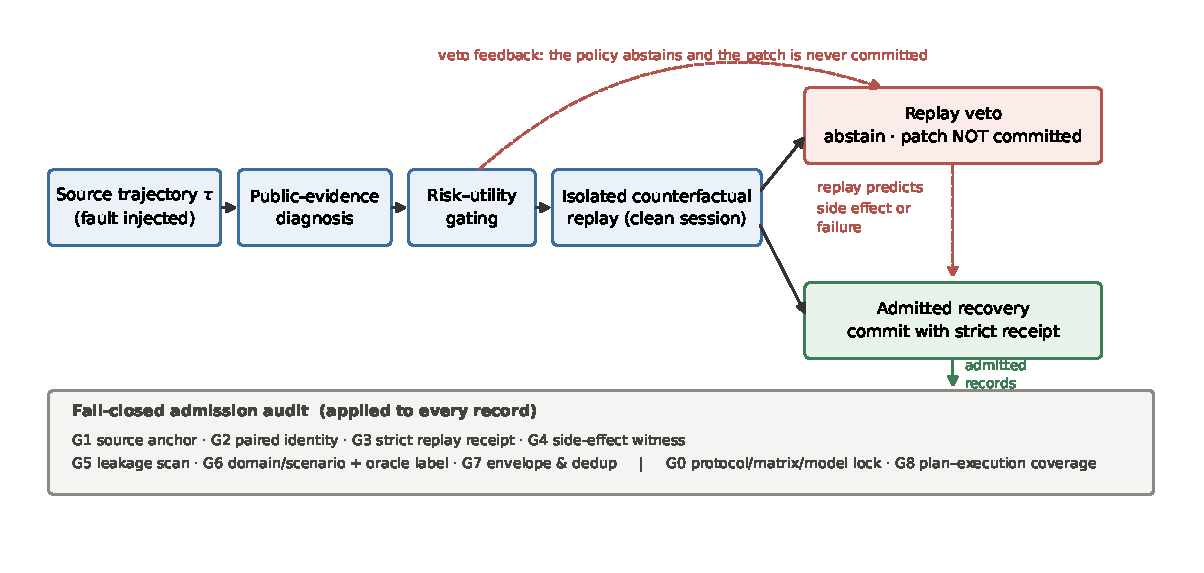
\includegraphics[width=\textwidth]{figures/fig1-racer-loop}
\caption{The RACER loop. A recovery claim passes through public-evidence diagnosis, risk--utility gating, and an isolated counterfactual replay. When the replay predicts a side effect or a failure, the policy vetoes the commit and abstains; otherwise the patch is committed with a strict replay receipt. Every admitted record must additionally pass the fail-closed admission audit (G1--G7 at record level; G0 and G8 at evaluator level).}
\label{fig:loop}
\end{figure}

Fig. 1 summarizes the loop: the four stages below correspond to Definitions 1--3, and the audit band shown at the bottom of the figure is detailed under \emph{Admission}.

\textbf{Diagnosis on public evidence.} The diagnoser scans the trajectory step by step: (i) a mismatch between the tool name of the requested and the effective action yields an \texttt{effective\_tool\_mismatch} candidate (covering the observable consequences of \texttt{wrong\_tool} and \texttt{replace\_action}); (ii) a tool error yields an \texttt{action\_error} candidate whose root cause is the error string (the injected error text embeds its fault type, e.g. "injected rate\_limit"); (iii) a constraint violation is traced back to the selection step. A key design constraint is that \textbf{semantic judgments are derived from public text only}: refundability candidates come from the task text and invariants rather than from hard-coded flight semantics. As disclosed in \S7, a first implementation hard-coded ``selecting F2 violates the constraint'' and produced 40 rows of false-positive harmful repairs on the non-refundable task variant; the defect was exposed by counterfactual replay (the replayed patch exhibited a side effect) and dropped to zero after the fix. That episode is itself evidence for the value of the closed loop.

\textbf{Policy: risk--utility gating.} Candidates are ranked by utility and the highest-utility candidate is turned into a patch: error-type candidates restore the \texttt{requested\_action} (retry semantics), argument-type candidates perform a substitution. The decision records the expected cost/risk and sets \texttt{use\_counterfactual = true}.

\textbf{Verification: isolated counterfactual replay and veto.} For each patch the replayer opens a \texttt{<run\_id>:cf} session with the source seed, an empty fault schedule, and the original intent restored via \texttt{requested\_action}, then executes the prefix--patch--suffix sequence. The session returns the trajectory, the evaluation, and \texttt{replay\_provenance} (valid/strict/source contract); the replayer independently recomputes the expected contract and compares it field by field. Per Definition 2, when the replay predicts a side effect or a failure the decision is changed to abstain and the patch is not committed. The \texttt{RACER$-$counterfactual} ablation skips the replay and \textbf{directly commits} the patch to the source environment, which lets us observe the real behavioral consequence of ``commit without verification''.

Every baseline has access to the replayer: it is a shared service, and whether to replay is a property of the policy under test rather than a privilege of RACER. The \texttt{RACER$-$counterfactual} ablation occupies exactly the complementary cell---it builds the same patches with the same access to that service but commits them directly---which is what licenses the 2$\times$2 decomposition to attribute the difference to verification rather than to availability of the side-effect oracle.

\textbf{Admission: fail-closed auditing.} The main table accepts only a canonical envelope that satisfies the following gates. \textbf{G1} anchors the source manifest by SHA-256. \textbf{G2} recomputes the paired identity from \texttt{task\_id} and the environment contract. \textbf{G3} requires every recovery claim to carry a valid and strict receipt whose expected contract recomputes identically; a claim without such a receipt is rejected outright, and the \texttt{racer\_no\_counterfactual} ablation therefore recovers exactly 0\%. \textbf{G4} requires a side-effect row to satisfy one of three forms. Under the \emph{refund-semantics} form the row carries a refund entity, a SHA-256 ledger witness and a positive integer ledger count. Under the \emph{replay-attested} form it carries \texttt{counterfactual\_supported} together with \texttt{replay\_valid} and a credential chain. Under the \emph{direct-application} form it carries \texttt{direct\_applied = true} and an immutable apply receipt issued by the environment, whose witness is the SHA-256 of the canonical JSON holding the sequence, tool, arguments, \texttt{state\_after\_hash}, success, side effect and run id; because the behavioral outcome lies inside the hashed material, a forged harmful claim is infeasible. This form retires the earlier self-reported boolean, and legacy tables written in that form return NO-GO under the upgraded auditor by design. \textbf{G5} applies key-name and value-pattern scanning to reject ground-truth or credential leakage. \textbf{G6} enforces domain and scenario identity together with the oracle label source for the current protocol version. \textbf{G7} checks the envelope shape, the field row whitelist, and a deduplication proof showing zero duplicates. On the evaluator side, \textbf{G0} locks the protocol, matrix and model resource, while \textbf{G8} enforces plan--execution coverage completeness, preflighted separately for each track. The gates are not a flat checklist but a mapping onto distinct threats: G5 guards against ground-truth leakage into agent-visible surfaces; G1 and G2 against identity substitution and cross-environment comparison; G3 against recovery claims that cannot be recomputed; G4 against forged or self-reported side-effect statements; G6 against label-provenance drift, since a harm label must originate in the oracle chain rather than in replay output; G0 and G8 against protocol, matrix and model drift between the plan and the execution; and G7 against envelope malformation and duplicate rows.

\section{Benchmark Design}

\textbf{Protocols and pre-registration discipline.} Every experiment follows a frozen protocol. Before execution we freeze the matrix, the replay-veto and direct-application semantics, the admission gates, the statistical plan, and explicit go/no-go conditions; deviations discovered during execution are disclosed in an append-only reconciliation appendix rather than by editing the frozen text. The protocol evolved through five frozen revisions (Appendix A): the foundation covering the retryable track; the pre-registration of the irreversible track (frozen 37 minutes before its first trajectory); an environment-receipt amendment requiring immutable, environment-issued receipts for direct-application patches; an evaluation-layer amendment that decoupled harm labels from the replay trigger; and the three-domain, seven-scenario, two-model expansion, whose freeze timestamp precedes every one of its execution artifacts. Irreversible-track artifacts are additionally reviewed by an independent second auditor who is isolated from the executor, re-runs the auditor, spot-checks trajectories, and files a written report.

\textbf{Three semantic domains.} The task environment implements three domains through a single engine with per-domain dispatch: flight (\texttt{search\_flights} / \texttt{select\_flight} / \texttt{confirm\_booking}), hotel (\texttt{search\_rooms} / \texttt{select\_room} / \texttt{confirm\_reservation}), and shop (\texttt{search\_products} / \texttt{select\_product} / \texttt{place\_order}). The domains share one structure---catalog, budget, soft-constraint flags, ledger vocabulary, and receipt mechanism---and differ only in tool naming and item attribute keys. The design goal is to make a unified harm predicate,

\[\text{harm} = \text{confirmed} \wedge \neg\text{optimal\_selection},\qquad \text{optimal} = \arg\min_{\text{price}} \{ \text{item} : \text{soft flag} \wedge \text{in stock} \wedge \text{price} \le \text{budget} \},\]

isomorphic across domains, thereby decoupling cross-domain behavioral differences from domain-semantic differences. The shop domain additionally enforces an \texttt{in\_stock} hard gate.

\textbf{The irreversible-side-effect scenario family (7 scenarios).} The track was expanded from 2 cells to 7 independent scenarios, enumerated over domain $\times$ misleading-evidence mode $\times$ trigger fault, with every pair of scenarios differing on at least two axes (Table 1):

\begin{table}[t]
\centering
\caption{The seven irreversible-side-effect scenarios, enumerated over domain, misleading-evidence mode, and trigger fault.}
\label{tab:2}
\begin{tabular}{llll}
\toprule
\# & Domain & Misleading evidence & Trigger fault \\
\midrule
S1 & flight & omission (the real optimum is absent from the listing) & \texttt{force\_error} at confirm \\
S2 & flight & price corruption (the optimum's price is inflated to the budget boundary) & \texttt{rate\_limit} at confirm \\
S3 & hotel & omission & \texttt{wrong\_tool} at confirm \\
S4 & shop & stock falsification (the optimum is reported out of stock) & \texttt{force\_error} at place order \\
S5 & hotel & stale quote (a non-optimal room is shown cheaper) & \texttt{rate\_limit} at confirm \\
S6 & shop & omission & \texttt{rate\_limit} at place order \\
S7 & flight & stale quote & \texttt{wrong\_tool} at confirm \\
\bottomrule
\end{tabular}
\end{table}


The four misleading-evidence modes are used 3, 1, 1 and 2 times respectively, the three trigger faults 2, 3 and 2 times, and the domain distribution is flight 3, hotel 2 and shop 2. Scenario legality is derived from engine semantics rather than chosen freely: a corrupted catalog can only steer the agent \emph{away from} the true optimum toward a ``committable but suboptimal'' item, because steering toward an item that is genuinely ineligible fails the confirm-time recheck and therefore cannot constitute a harmful commit. Three mechanisms were excluded after analysis because they carry no trap value: \texttt{drop\_action} is a silent no-op with no visible failure (all baselines abstain, no separation), response loss makes the source terminal state harmful for every strategy, and a mis-planned ground-truth listing lets RACER recover correctly. Scenarios are frozen and computationally validated before execution: a registry fixes task identities, catalogs, fault schedules, and classification directions, and a pairwise axis check plus regression tests re-assert independence.

\textbf{The retryable-fault track.} A fault matrix (five fault types injected at the confirmation step) $\times$ 5 seeds, together with task variants (clean success, non-refundable, suboptimal-refundable, missing confirmation, force-error-at-confirm, dropped confirm) $\times$ 5 seeds, gives 11 cells $\times$ 10 seeds per domain after expansion. Every cell enables an idempotent refund ledger (\texttt{refund\_booking} is idempotent and emits a SHA-256 ledger witness, with a \texttt{get\_refund\_status} reconciliation query), so that any side-effect claim naturally satisfies the refund-semantics form of G4.

\textbf{Baselines (14, executed in pairs).} \emph{No repair:} \texttt{raw\_react}. \emph{Retry family (2):} \texttt{fixed\_retry}, \texttt{exponential\_backoff}. \emph{Diagnosis family (5):} \texttt{generic\_reflection}, \texttt{full\_trace\_judge} (which requires corroboration from multiple candidates), \texttt{step\_by\_step\_diagnosis}, \texttt{binary\_search\_diagnosis}, \texttt{agentdebug\_targeted\_feedback}. \emph{Ablations:} \texttt{always\_recover}, \texttt{racer}, \texttt{racer\_no\_abstain}, \texttt{racer\_no\_counterfactual} (commits patches directly, never calls the replayer, and by construction has \texttt{counterfactual\_supported = false}). \emph{Oracle upper bounds:} \texttt{oracle\_root\_cause} (ground-truth step plus a public-evidence patch) and \texttt{oracle\_recovery} (repairs only when ground truth contains an explicit patch). Oracles receive ground truth through a privileged channel; every other baseline sees only the public trajectory.

\textbf{Model resources and execution.} The primary model is \texttt{oneapi-relay-glm-5.3-flash} (Anthropic-native \texttt{/v1/messages} with \texttt{tool\_use}; temperature 0.0) and the replication model is \texttt{oneapi-relay-deepseek-v4-flash} (same protocol, same registry discipline). A revision lock anchors the actor source, system prompt, tool schema, sampling parameters, and code commit. The relay's Claude node suffered sustained HTTP 529 overload; per a pre-registered substitution clause we switched to a same-protocol GLM node and disclose this as a validity threat in \S7. Credentials are injected only through runtime environment variables and never enter the repository or the artifacts. The actor is capped at 6 steps on the main track (episodes complete in 2) and 8 steps on the irreversible track (episodes complete in 3); an episode ends at confirmation, at actor termination, or at a tool error; because the runner fails fast, retryable faults become persistent failures (see \S6.6). The execution matrix comprises 330 main-track episodes (3 domains $\times$ 11 cells $\times$ 10 seeds, 4,620 records per model) and 70 irreversible-track episodes (7 scenarios $\times$ 10 seeds, 980 records per model), i.e. 800 episodes and 11,200 records across the two models. v0.5 additionally repairs a step-position defect inherited from the first protocol version, in which confirmation-position faults were scheduled at a step the 2-step actor never reached; faults were remapped and a behavioral probe confirmed that they now fire.

\textbf{Statistical procedure (pre-registered).} Wilson 95\% intervals are descriptive. Paired comparisons encode a three-way outcome per episode (+1 harmless recovery / 0 no recovery / $-$1 harmful repair); paired differences are evaluated with 10,000 stratified cluster-bootstrap resamples and 10,000 sign permutations under fixed seeds, and the primary family (RACER vs. the 11 non-oracle baselines) is corrected with Holm--Bonferroni at $\alpha$ = 0.05. For the irreversible track the pre-registered hypothesis family is a two-item Holm family: \textbf{H-E3a} (harm rate, episode-cluster bootstrap plus permutation) and \textbf{H-E3b} (veto accuracy, exact binomial). Results are stratified by domain $\times$ scenario $\times$ model. The Mantel--Haenszel common odds ratio is reported descriptively only (with a Haldane--Anscombe correction for zero cells and an explicit caveat that its confidence interval is uninformative there). Cross-model pooling is executed \textbf{only if} both models agree on the direction in all seven scenarios (Q.3); cross-domain differences are descriptive only, since three domains cannot support a between-domain significance claim (Q.4). A pre-registered caution notes that the irreversible track is a mechanistic verification track, so the main significance claim rests on the stratified tests rather than on a single aggregate.

\section{Results}

\textbf{Overview.} Under the frozen protocol we executed both tracks with both models: 1,960 records on the irreversible track (7 scenarios $\times$ 10 seeds $\times$ 14 baselines $\times$ 2 models) and 9,240 records on the main track (3 domains $\times$ 11 cells $\times$ 10 seeds $\times$ 14 baselines $\times$ 2 models). Every record passes the admission auditor (G1--G7, including the domain/scenario identity and oracle-label gates), with an exclusion rate of 0\%; the plan--execution coverage check passes on all four matrices, version-regression audits remain green, and the direction-consistency gate is satisfied in all seven scenarios under both models (14 of 14 scenario--model combinations). Under the stricter pre-registered separation rule, which requires a full 100\% harmful-commit rate from the seven non-verifying baselines other than the full-trace judge, 12 of the 14 combinations qualify; the two shortfalls are DeepSeek S5 and S7, where part of the source episodes never reached the failure denominator (\S6.4). We exclude the judge from that rule because its abstentions are a deterministic property of the baseline (it requires corroborating trace evidence that injected errors do not leave) and replicate across both models; including it would make the rule measure the baseline's abstention behavior rather than the separation of strategies.

\subsection{Main track: three domains, two models, 9,240 records}

The main track contains no irreversible trap---its purpose is to measure recovery rate and domain generality---so harm is zero by design for every baseline on every domain and model, and the evidentiary weight of harm separation rests entirely on the irreversible track. Table 2 reports verified recovery per domain and model, together with the within-domain paired comparisons of RACER against the three most informative baselines.

\begin{table}[t]
\centering
\caption{Main-track verified recovery and within-domain paired tests. Recovery is reported over the episodes that failed in the source environment; each domain contributes 110 episodes per model (failures: GLM 41/47/23, DeepSeek 9/24/36 for flight/hotel/shop). The last three columns give the within-domain permutation $p$ against the no-verification ablation, the no-repair baseline and the full-trace judge, and harm over all 1,540 baseline rows per domain and model.}
\label{tab:3}
\begin{tabular}{lllll}
\toprule
Domain & Model & Verified recovery & Paired $p$ vs. \texttt{no\_cf} / \texttt{raw} / \texttt{judge} & Harm (all baselines) \\
\midrule
flight & GLM & 41/41 (100\%) & 0.0001 / 0.0001 / 0.0001 & 0/1540 \\
hotel & GLM & 47/47 (100\%) & 0.0001 / 0.0001 / 0.0001 & 0/1540 \\
shop & GLM & 18/23 (78.3\%) & 0.0001 / 0.0001 / 0.0008 & 0/1540 \\
flight & DeepSeek & 9/9 (100\%) & 0.0039 / 0.0044 / 0.0342 & 0/1540 \\
hotel & DeepSeek & 24/24 (100\%) & 0.0001 / 0.0001 / 0.0012 & 0/1540 \\
shop & DeepSeek & 27/36 (75.0\%) & 0.0001 / 0.0001 / 0.0001 & 0/1540 \\
\bottomrule
\end{tabular}
\end{table}


Within each domain the Holm family consists of RACER against the 11 non-oracle baselines. In GLM, all three domains reject the null for the no-verification ablation, the no-repair baseline, and the full-trace judge (Holm-adjusted $p \le 0.008$). In DeepSeek, hotel and shop reject for all three, while flight rejects for the no-verification and no-repair baselines (Holm-adjusted $p$ = 0.043 and 0.044) but not for the full-trace judge (Holm-adjusted $p$ = 0.308, because the raw $p$ of 0.034 does not survive correction across an 11-item family). Against the retry-family baselines the difference is exactly zero in every domain and both models ($p = 1.0$)---a null result that mirrors the retryable-track finding of \S6.6: the differential benefit of verification lives in the harmful dimension, not in the retryable one.

Three structural observations follow.

\begin{enumerate}

  \item \textbf{A cross-domain recovery gap (shop, 75--78\%).} The \texttt{in\_stock} hard gate in the shop domain means that for a subset of fault cells the optimal item has become unreachable by the time recovery is attempted (its stock is consumed by the preceding action). The replay truthfully predicts that the item reachable by the patch is not optimal, and the policy vetoes rather than committing a suboptimal choice. This is a faithful reflection of \emph{domain semantics}: RACER behaves consistently in all three domains, and the gap originates in environmental reachability rather than in framework failure. The gap replicates across models (GLM 78.3\%, DeepSeek 75.0\%).

  \item \textbf{No difference against the retry family on the main track.} With no trap in the design, retrying is the correct repair, so verification and naive retrying coincide---consistent with the earlier retryable-track finding.

  \item \textbf{A large-scale test of the fail-closed declaration semantics.} In the GLM main track, 106 rows of the no-verification ablation applied a patch directly and succeeded behaviorally with a valid environment receipt, yet were normalized to \emph{unverifiable} recovery because they carry no replay receipt; in the DeepSeek main track the count is 60 (\S6.4). After this normalization both models recover 0\% for the ablation---identical to the encoding used in earlier protocol versions. The normalization is a statement about declaration semantics rather than a data correction: \emph{unverified recovery does not count as recovery}, which is the paper's central claim.

\end{enumerate}

\subsection{Irreversible-side-effect track: seven scenarios, two models}

\begin{figure}[t]
\centering
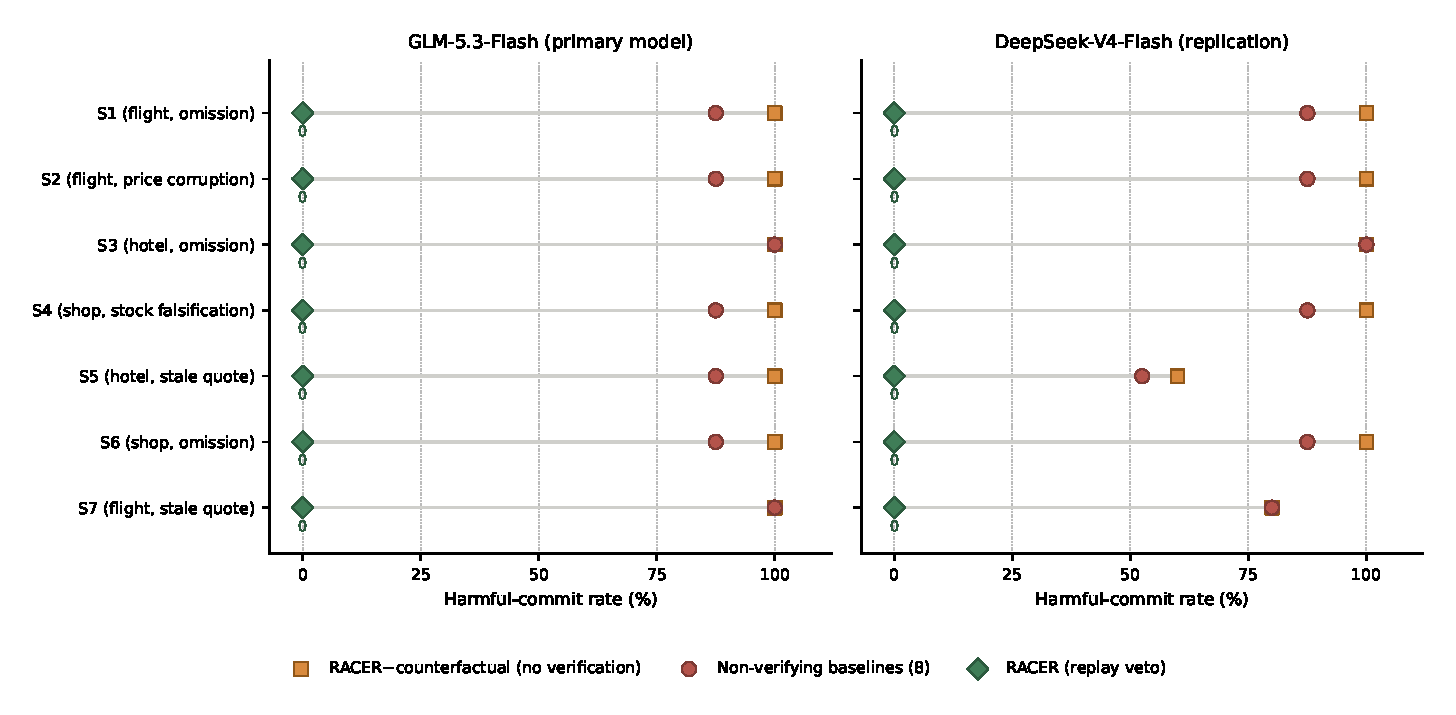
\includegraphics[width=\textwidth]{figures/fig2-scenario-separation}
\caption{Behavioral separation on the irreversible-side-effect track, per scenario and model. Each scenario shows the harmful-commit rate of the retry family (8 baselines, 80 rows per scenario) and of the unverified ablation RACER$-$counterfactual (10 rows per scenario) against RACER (10 rows per scenario), whose harmful-commit rate is zero in every scenario under both models. Exact rates are plotted without error bars.}
\label{fig:sep}
\end{figure}

All episodes on this track fail in the source environment by construction. \textbf{Table 3} reports the joint harmful-commit rate of the eight non-verifying baselines---the retry family, the diagnosis family and \texttt{always\_recover} (denominator 80 = 8 baselines $\times$ 10 seeds) and the veto-abstention rate of the two RACER baselines (denominator 20), per scenario and model.

\begin{table}[t]
\centering
\caption{Behavioral separation on the irreversible-side-effect track.}
\label{tab:5}
\begin{tabular}{llllll}
\toprule
\# & Domain / misleading evidence / trigger & Non-verifying harm (GLM) & RACER veto abstain (GLM) & Non-verifying harm (DS) & RACER veto abstain (DS) \\
\midrule
S1 & flight / omission / \texttt{force\_error} & 70/80 & 20/20 & 70/80 & 20/20 \\
S2 & flight / price@boundary / \texttt{rate\_limit} & 70/80 & 20/20 & 70/80 & 20/20 \\
S3 & hotel / omission / \texttt{wrong\_tool} & 80/80 & 20/20 & 80/80 & 20/20 \\
S4 & shop / stock falsification / \texttt{force\_error} & 70/80 & 20/20 & 70/80 & 20/20 \\
S5 & hotel / stale quote / \texttt{rate\_limit} & 70/80 & 20/20 & 42/80 & 16/20 \\
S6 & shop / omission / \texttt{rate\_limit} & 70/80 & 20/20 & 70/80 & 20/20 \\
S7 & flight / stale quote / \texttt{wrong\_tool} & 80/80 & 20/20 & 64/80 & 18/20 \\
\bottomrule
\end{tabular}
\end{table}


\emph{Reading the table.} Every non-verifying row short of the full score is attributable to the full-trace judge, which requires corroboration from multiple candidates and therefore abstains deterministically when the injected error leaves no corroborating trace evidence (the \texttt{force\_error} and \texttt{rate\_limit} families). This is a \textbf{baseline design property rather than model noise}: the same pattern predates the current protocol version, was known from the pre-execution smoke test, and replicates across models. Under a pre-registered deviation rule that permits up to three deviating scenario--model combinations out of fourteen, and which is evaluated over the seven non-verifying baselines other than the judge itself, these abstentions are treated as a baseline-level systematic deviation and are disclosed and analyzed separately (\S6.4, \S7). In the \texttt{wrong\_tool} family (S3, S7) the judge instead retries and falls into harm, so those two scenarios reach the full score. The two DeepSeek rows that fall further short (S5 at 42/80 and S7 at 64/80) have an additional model-level cause: in some trials the source episode never reached the tool-error failure denominator because the actor stalled and exhausted its step budget. These constitute the two disclosed deviations within the pre-registered quota.

\textbf{Primary hypotheses (two-item Holm family).}

\begin{itemize}

  \item \textbf{H-E3a (harm rate).} The family-minus-RACER difference in harm rate is 0.911 with CI [0.898, 0.923] and $p = 1\times10^{-4}$ for GLM, and 0.832 with CI [0.766, 0.888] and $p = 1\times10^{-4}$ for DeepSeek; both models reject the null after Holm correction.

  \item \textbf{H-E3b (veto accuracy).} GLM reaches 70/70 (exact binomial $p = 2^{-70}$) and DeepSeek 64/70 (91.4\%, $p = 1.2\times10^{-13}$); both reject after Holm correction. The six incorrect vetoes of DeepSeek are concentrated in S5 (four) and S7 (two) and correspond to the misalignment described above, where the source episode never failed, so an abstention on a non-failing episode cannot be counted as a correct veto. They are not harmful patches that the veto failed to catch: in the harm dimension neither model leaks a single case (RACER harm is 0/140 in both).

  \item \textbf{Resolution of the tests.} Both permutation $p$-values sit at $1\times10^{-4}$, the floor of a 10,000-sample permutation test, so they should be read as ``at least this small'' rather than as exact values; the bootstrap confidence intervals, which do not depend on permutation resolution, carry the effect size.

  \item \textbf{Directional consistency.} In both models, 7 of 7 scenarios show a higher non-verifying harmful-commit rate than RACER's harmful-commit rate.

  \item \textbf{No-verification ablation.} Committing patches without replay is harmful in 70/70 cases for GLM and 64/70 for DeepSeek (with the S5 and S7 shortfalls again attributable to the same denominator effect).

\end{itemize}

Both models agree in direction on all seven scenarios, which satisfies the pre-registered condition for cross-model pooled stratified analysis. Fig. 2 visualizes the same separation for all seven scenarios and both models, together with the unverified ablation.

\subsection{Independent oracle recomputation of harm labels}

An earlier protocol version contained a circularity that we removed by an evaluation-layer amendment (execution evidence frozen, no re-execution). Previously the harm label (read by the evaluator from the replay session's \texttt{evaluate().side\_effect}) and the replay-veto trigger (read by the runner from the same \texttt{evaluate().side\_effect}) consumed \textbf{the same boolean}, so the statement ``the verification layer prevented harmful commits'' was partly definitional. The amendment decouples them:

\begin{itemize}

  \item \textbf{Independent label chain.} Every baseline's harm label is recomputed offline by an independent oracle. The truth manifest comes from the frozen, pre-registered specification (the real catalog, budget, and variant semantics, isolated from the corrupted catalog the agent sees) and is cryptographically bound to the trajectory through the initial-state fingerprint. The recomputation consumes only the trajectory's raw behavioral evidence (the observation state and the per-step state hash chain) and \textbf{never reads any evaluation output}; its predicate is an independent rewrite of the environment's evaluation and shares no code. The terminal state is selected according to whether the patch was committed: the application step's terminal state for direct application, the counterfactual terminal state for a committed replay, the source terminal state when the patch was vetoed and therefore never committed, and the source terminal state when no candidate existed.

  \item \textbf{Zero label flips.} The independent oracle reproduces the environment label for \textbf{every} row of the current matrix---1,960 irreversible-track rows and 9,240 main-track rows across both models---so the behavioral separation holds under independent ground truth rather than by definition.

  \item \textbf{Veto accuracy.} Every veto's predicted path is recomputed by the oracle as a genuinely harmful terminal state: the veto never wrongly blocked a harmless patch and never let a harmful one through, which the model-specific accuracy figures of \S6.2 quantify.

  \item \textbf{Labels, not numbers, changed.} Because labels do not flip, all statistics are unchanged relative to the previous version; what changed is the \emph{way labels are proven}. Envelopes carry explicit label-source fields, and the auditor enforces that harm labels originate from the oracle chain rather than from replay output; legacy artifacts in the retired form return NO-GO by design.

  \item \textbf{Disclosure.} The amendment's freeze timestamp is later than a same-day trial run over frozen trajectories that was used to validate the oracle implementation's feasibility; the rule text was not edited retroactively, and the ordering is disclosed in the protocol document.

  \item \textbf{Extension to three domains.} The independent chain is parameterized to all three domains, with the flight path byte-identical to the earlier version and hotel/shop added isomorphically; the label source is enforced by an admission gate for the current protocol version.

\end{itemize}

\subsection{Cross-model replication and disclosed model-level deviations}

The replication model reproduces the core pattern of behavioral separation exactly: RACER harm is zero in every scenario, the veto-abstention pattern is identical, and the full-trace judge's abstention pattern recurs scenario by scenario (S1, S2, S4 and S6 at 70/80 in both models). Model-level differences are disclosed as follows.

\begin{enumerate}

  \item \textbf{Failure-denominator differences.} The DeepSeek actor exhibits more multi-step behavior (223 step-budget exhaustions versus 147 for GLM), so in four of ten S5 trials and in a subset of main-track fault cells the source episode never reached the tool-error failure denominator---the fault was injected, but the episode ended in an actor stall. This compresses the DeepSeek retry-family denominator in S5 (42/80) and does not threaten the direction of separation: RACER is strictly less harmful than the non-verifying baselines in all 14 scenario--model combinations, and 12 of the 14 still satisfy the stricter pre-registered separation rule (which allows at most three shortfalls).

  \item \textbf{Direct-application frequency differs across models.} The no-verification ablation applied a patch directly in 106 rows under GLM and 60 rows under DeepSeek, reflecting how often each actor's diagnostic output yielded an applicable patch on those cells. Both models nonetheless report 0\% verified recovery for that ablation, because the fail-closed declaration semantics refuse a recovery claim that carries no replay receipt; the ablation conclusion is therefore unaffected.

  \item \textbf{Execution-coverage disclosure.} The two models share frozen run identifiers by matrix design, so the later-executed model overwrites the trajectory files on the shared volume; the earlier model's envelopes had already been built and persisted, and complete traces are retained in the run JSON, so reproducibility is unaffected.

\end{enumerate}

\subsection{Ablation: a 2$\times$2 decomposition of gating and verification}

Table 4 decomposes the harmful-commit rate on the irreversible track along two components---risk--utility gating and counterfactual-replay verification---using the 7 scenarios $\times$ 10 seeds $\times$ 2 models matrix.

\begin{table}[t]
\centering
\caption{Two-by-two ablation on the irreversible track.}
\label{tab:6}
\begin{tabular}{llllll}
\toprule
Gating & Verification & Baseline & Harm (GLM) & Harm (DeepSeek) & Verified recovery (main track) \\
\midrule
\checkmark{} & \checkmark{} & RACER & 0/70 & 0/70 & Table 2 \\
$\times$ & \checkmark{} & RACER$-$abstain & 0/70 & 0/70 & Table 2 \\
\checkmark{} & $\times$ & RACER$-$counterfactual & 70/70 & 64/70 & 0\% \\
$\times$ & $\times$ & \texttt{fixed\_retry} (retry-family representative) & 70/70 & 64/70 & Table 2 \\
\bottomrule
\end{tabular}
\end{table}


The conclusion is that \textbf{replay verification is a behaviorally necessary component for preventing harmful commits}: every policy that carries the verification layer commits zero harmful repairs, whereas every policy that lacks it---including the gated but unverified ablation and including the oracle root-cause baseline---commits harmful repairs at scale in both models. (The DeepSeek shortfall to 64/70 again originates in six trials that never reached the failure denominator, not in protection by the verification layer.) Gating by itself does not prevent a harmful commit, as the identical rates of the unverified ablation and \texttt{fixed\_retry} demonstrate; its contribution is declaration discipline and abstention policy. The other half of the recovery claim is captured by the fail-closed declaration semantics: a recovery without a receipt is never admitted; the unverified ablation consequently recovers 0\% on the main track. Its harmful commits are attested by an environment-issued receipt rather than by a self-reported boolean, and the harm labels themselves are cross-attested by an oracle that never reads replay output---so behavior, declaration, and ground truth provide three mutually independent layers of evidence for the necessity of the verification layer.

The comparison against \texttt{raw\_react} deserves emphasis, because it bounds the claim. \texttt{raw\_react} is also harmless on the irreversible track---doing nothing cannot commit a harmful repair---so RACER's advantage there is not harm avoidance alone. What distinguishes the two is the joint behavior: the same policy recovers on the retryable track, where \texttt{raw\_react} recovers nothing while RACER recovers every failure-eligible episode in all three domains and both models (Table 2). An unconditional abstainer would match RACER's harm count on the irreversible track while forfeiting every recoverable failure; the contribution is therefore the combination of verified recovery and verified refusal, not abstention by itself.

\subsection{Failure structure and self-healing}

Three structural observations characterize the gap between ``a fault was injected'' and ``a persistent failure occurred''.

\begin{enumerate}

  \item \textbf{\texttt{drop\_action} and \texttt{replace\_action} are self-healed.} In all ten affected cells the original episode succeeded: the dropped or replaced confirmation step returned \texttt{ok = true}, the episode did not terminate, and the LLM actor observed an unconfirmed state on its next turn and naturally re-issued the confirmation. The fault occurred but was absorbed by agent behavior.

  \item \textbf{Variant faults scheduled at the third step were never reached} in the earliest protocol version, because the actor completed those tasks in two steps (the listing is visible in the observation, so no search step is needed) and the injection point was never visited. The current protocol remaps those faults and verifies with a behavioral probe that they fire.

  \item \textbf{Persistent failure requires fail-fast $\times$ retryability.} The retryable-track failures are exactly those where a tool returned an error and the runner terminated immediately while a retry would have repaired the fault; the irreversible-track failures are those where a retry succeeds but commits a suboptimal decision. The two classes are orthogonal and together form the failure denominator.

\end{enumerate}

The methodological implication for fault-injection benchmarks is that \textbf{a fault must interact with the agent policy and be reinforced by the environment through either termination or irreversibility in order to constitute a valid failure denominator}; otherwise the failure rate is systematically underestimated and the recovery rate overestimated. The cross-model execution adds a second face to this implication: because the DeepSeek actor's multi-step behavior leaves some injected faults below the tool-error termination threshold, the failure denominator is itself a joint product of \emph{model policy} and \emph{termination semantics}, and cross-model comparisons must therefore be stratified by model.

\subsection{Cost}

Across the full two-model matrix (800 episodes) the study issued 2,118 LLM calls and consumed approximately 1.94 million tokens: 212 calls / 49,980 tokens on the GLM irreversible track (21.1 s per episode), 813 / 500,797 on the GLM main track (32.4 s), 209 / 262,757 on the DeepSeek irreversible track (8.8 s), and 884 / 1,123,149 on the DeepSeek main track (7.0 s). DeepSeek consumes roughly 2.3$\times$ the tokens of GLM---consistent with its longer chain-of-thought output and multi-step behavior---while its latency is about one quarter. The call-ledger conservation invariants hold in every episode (zero invalid actions, one endpoint error on the GLM main track that was recovered by retry, and seven empty-tool-use events absorbed by the in-protocol retry mechanism, none of which fabricated an action). An execution-time truncation defect of the GLM thinking block (an empty content caused by exhausting the token budget inside the thinking block) was repaired by raising the budget and applying a temperature ramp on empty-content retries; the defect and its fix are recorded in the model registry.

\subsection{A negative result on the $\tau^{2}$-airline adaptation}

Adapting the native $\tau^{2}$-airline environment (pilot tier) produced a G4 failure: its refund operation is non-idempotent, exposes no publicly recomputable ledger witness, and therefore cannot satisfy the admission audit for a side-effect claim. This negative result directly motivated the idempotent-ledger design of our own environment and illustrates the hardening value of fail-closed auditing for external benchmarks: \textbf{an unauditable side-effect semantics makes any recovery claim untrustworthy}.

\section{Limitations and Threats to Validity}

\textbf{Scope.} The study covers three domains (implemented by a single engine with per-domain dispatch), three candidate actions, and trajectories of two to eight steps, with two LLM actors (GLM-5.3-Flash as the primary analysis and DeepSeek-V4-Flash as an independent replication) executed over the same protocol. The irreversible-side-effect track (7 scenarios $\times$ 140 episodes per model) is a mechanistic verification track whose purpose is to test the constructive proposition ``harm exists and can be vetoed''; it is not designed to estimate an overall effect size. Rates such as 100\% and 0\% should not be extrapolated to production agents, and every quantitative conclusion is bounded by this matrix. The three-domain recovery gap in the shop domain originates in environmental reachability under the \texttt{in\_stock} gate rather than in framework failure, and three domains cannot support a between-domain significance claim, so domain differences are reported descriptively only. A step-position defect in the earliest protocol version (confirmation-position faults that a two-step actor never reached) was repaired in the current version and disclosed at pre-registration; the earliest numbers are retained and labeled as ``fault not activated''.

\textbf{Track complementarity.} On the retryable track, RACER and naive retrying are indistinguishable, and this replicates across all three domains and both models. This null result and the total separation on the irreversible track jointly define the claim: the differential benefit of verification lies in the harmful dimension, not in the retryable one. The direction of separation was pre-registered, which lowers its surprise value; the mechanistic evidence (the original decisions behind each veto, the direct-application receipts, and the cross-model replication of separation in 12 of 14 combinations) together with the audit chain is the primary support. The abstention of the full-trace judge in the \texttt{force\_error} and \texttt{rate\_limit} families is a baseline design property (the judge requires corroboration and injected errors leave none), confirmed as non-model-specific by cross-model replication, and is handled as a disclosed deviation under the pre-registered rule; the two deviating DeepSeek scenario--model combinations (S5 and S7, where the source episode never reached the failure denominator) fall inside the pre-registered quota and are itemized above.

\textbf{Validity and infrastructure.} (i) A mid-project model substitution (Claude $\to$ GLM-5.3-Flash, caused by relay overload) occurred after the protocol freeze, was executed under a pre-registered substitution clause, and is disclosed; results are not comparable with the originally planned model. (ii) A temperature ramp on empty-content retries (+0.1 per attempt, capped at 0.7) deviates from the locked temperature of 0.0; it never fired in the final runs and is retained only as a validated defense. (iii) A semantic hard-coding defect in the first diagnoser implementation (\S4) produced 40 false-positive harmful repairs in the first full run; after the fix and a full re-run the count returned to zero. The main table comes from the post-fix run and the defective data is archived---this is simultaneously a threat (a first version released as-is would have reported wrong conclusions) and evidence that the closed loop caught it. (iv) The irreversible-track execution used a revised actor (raised token budget, suppressed repeated search); the revision preceded that run and is registered, but an engineering difference exists between protocol versions. (v) A process deviation occurred once: an early matrix upgrade was not written back into the protocol text before execution; later revisions therefore introduced the pre-registration plus second-auditor discipline; subsequent matrix changes have frozen a new protocol version before execution. (vi) The first execution of the irreversible track expressed direct application through a self-reported boolean, a low-risk gameable surface flagged by the auditor; a later amendment closed it with environment-issued receipts and re-ran the track, with per-baseline behavior identical across the two executions. (vii) The replication model's execution chain required one relay-adapter compatibility patch (its adapter requires a non-standard identifier field on assistant tool-use blocks); the patch is registered and disclosed here. (viii) The two models share frozen run identifiers, so the later-executed model overwrites trajectory files on the shared volume; the earlier model's envelopes had been built and persisted beforehand and full traces are retained in the run JSON.

\textbf{Deployment preconditions.} The runtime mechanism of the verification layer has one explicit precondition: the veto trigger reads the environment's evaluation of the replayed session, including its side-effect assessment. Therefore \textbf{the deployment environment must be able to assess side effects inside a controlled replay session}. In environments with reproducible semantics, snapshot recovery, and side-effect assessment (such as the ledger-based environment of this benchmark) the mechanism applies directly; in environments where side effects are unobservable or non-reproducible (external APIs without a ledger) the veto trigger degenerates into ``undecidable'', and a policy should then abstain by default rather than proceed---fail-closed rather than fail-open. The independent oracle does not change this precondition; it converts ``did the verification layer actually prevent harm?'' from a definitional question into an empirically recomputable one. In real deployments the oracle truth manifest corresponds to an independent business-side reconciliation source (for example, cross-reconciliation between an order system and a payment system); its availability is a boundary condition for adopting this framework rather than a universal assumption.

\textbf{Statistics.} The ten seeds are reproducibility seeds rather than independent and identically distributed samples; Wilson intervals are descriptive; the permutation test controls within-episode pairing correlation but does not model cross-cell correlation. The fail-closed declaration semantics make part of the ablation's 0\% recovery a matter of \emph{inadmissibility of the claim} on the retryable track; the irreversible track supplies the complementary behavioral evidence (real harmful commits in the direct-application form), but readers comparing numbers across papers should be aware of this convention.

\textbf{Robustness of the conclusions.} Despite these boundaries, the central claim---that the verification layer makes recovery claims auditable, is behaviorally necessary on irreversible faults, and is feasible under real LLM execution---rests on four independent lines of evidence: the stratified significance on the irreversible track in both models (H-E3a and H-E3b both Holm-rejected, with 7/7 directional agreement triggering the pre-registered pooled analysis), the 2$\times$2 behavioral separation over 1,960 rows and two models, the false-positive capture in the first run, and the negative G4 result on an external benchmark. Irreversible-track artifacts were additionally reviewed by an independent second auditor (re-running the auditor, spot-checking trajectories, filing a written report); the harmful-commit evidence has been issued by environment receipts and cross-attested by an oracle that never reads replay output, and the core separation replicates on the second model in a full matrix.

\section{Conclusion}

RACER reframes agent recovery from an observed coincidence into an auditable assertion: a recovery succeeds only if it is proven by an isolated counterfactual replay, anchored by a paired identity, and admitted by a fail-closed audit; when the replay predicts harm, the policy vetoes the commit and explicitly abstains. On a real-LLM benchmark of 800 episodes, 14 baselines, two models, and 11,200 records across three domains and two tracks, every record passed admission auditing with zero exclusions. On retryable faults RACER and naive retrying are indistinguishable---a null result. On irreversible side-effect faults (7 scenarios $\times$ 3 domains) unverified policies, including oracle root-cause repair, commit harmful repairs at scale in both models, whereas RACER's replay veto converts every case into harmless abstention (0/140 in each model); both hypotheses are Holm-significant in both models with 7/7 directional agreement, which triggers the pre-registered cross-model pooled analysis. The three-domain main table exposes a reachability gap under the shop domain's \texttt{in\_stock} gate: the framework behaves consistently across domains and the gap is explained by environmental semantics rather than framework failure. We also report a null result against the verification-preserving ablation, whose gating changes abstention rates but not outcome encoding, and the self-healing of injected drop/replace faults; together these delineate the evidential boundaries of each component. Future work includes broader model families and deployment validation in real production environments, parameterized families of irreversible faults (monetary gradients, multi-step irreversible chains), and the release of the fail-closed auditor and pre-registration discipline as standalone tooling that can serve as reusable, claim-level evidence infrastructure for agent-recovery research.

\section*{Competing interests}
The authors declare that they have no competing interests.

\section*{Data availability}
The frozen protocols, the execution reconciliation appendices, the matrices, the model-resource registry (without credentials), the baseline registry, and all artifacts---including the 800 trajectories, oracle manifests, evaluation outputs, the 11,200-record envelopes, the admission and version-regression audit JSON files, the statistical outputs, and the independent second-auditor report---are released with the paper. The implementation uses the Python standard library only and passes 229 unit tests. Credentials are injected exclusively through runtime environment variables and never enter the repository or the artifacts; public trajectories and evaluation ground truth are physically separated, and \texttt{fault\_truth} never appears in any agent-visible interface. Reproduction entry points and the command sequence are documented in the project README.

\begin{thebibliography}{99}
\bibitem{ref1} Zhu K, et al. Where LLM agents fail and how they can learn from failures. arXiv:2509.25370, 2025
\bibitem{ref2} Zhang S, Yin M, Zhang J, et al. Which agent causes task failures and when? On automated failure attribution of LLM multi-agent systems. In: Proceedings of the 42nd International Conference on Machine Learning (ICML), 2025: PMLR 267: 76583--76599. arXiv:2505.00212
\bibitem{ref3} Ma X, et al. Demystifying the lifecycle of failures in platform-orchestrated agentic workflows. arXiv:2509.23735, 2025
\bibitem{ref4} Zhang G, et al. AgenTracer: Who is inducing failure in the LLM agentic systems? In: International Conference on Learning Representations (ICLR), 2026. arXiv:2509.03312
\bibitem{ref5} Bonagiri A, et al. CausalFlow: Causal attribution and counterfactual repair for LLM agent failures. arXiv:2605.25338, 2026
\bibitem{ref6} Yao S, et al. $\tau$-bench: A benchmark for tool-agent-user interaction in real-world domains. In: International Conference on Learning Representations (ICLR), 2025. arXiv:2406.12045
\bibitem{ref7} Debenedetti E, Zhang J, Balunovic M, et al. AgentDojo: A dynamic environment to evaluate prompt injection attacks and defenses for LLM agents. In: Advances in Neural Information Processing Systems 37 (NeurIPS), Datasets and Benchmarks Track, 2024: 82895--82920. DOI: 10.52202/079017-2636
\bibitem{ref8} Ralph P, et al. Empirical standards for software engineering research. arXiv:2010.03525, 2020
\bibitem{ref9} Nosek B A, Ebersole C R, DeHaven A C, Mellor D T. The preregistration revolution. Proceedings of the National Academy of Sciences, 2018, 115(11): 2600--2606. DOI: 10.1073/pnas.1708274114
\bibitem{ref10} Yao S, Zhao J, Yu D, et al. ReAct: Synergizing reasoning and acting in language models. In: International Conference on Learning Representations (ICLR), 2023. arXiv:2210.03629
\bibitem{ref11} Shinn N, Cassano F, Gopinath A, et al. Reflexion: Language agents with verbal reinforcement learning. In: Advances in Neural Information Processing Systems (NeurIPS), 2023. arXiv:2303.11366
\bibitem{ref12} Madaan A, Tandon N, Gupta P, et al. Self-Refine: Iterative refinement with self-feedback. In: Advances in Neural Information Processing Systems (NeurIPS), 2023. arXiv:2303.17651
\bibitem{ref13} Schick T, Dwivedi-Yu J, Dess\'i R, et al. Toolformer: Language models can teach themselves to use tools. In: Advances in Neural Information Processing Systems (NeurIPS), 2023. arXiv:2302.04761
\bibitem{ref14} Qin Y, Liang S, Ye Y, et al. ToolLLM: Facilitating large language models to master 16000+ real-world APIs. In: International Conference on Learning Representations (ICLR), 2024. arXiv:2307.16789
\bibitem{ref15} Liu X, Yu H, Zhang H, et al. AgentBench: Evaluating LLMs as agents. In: International Conference on Learning Representations (ICLR), 2024. arXiv:2308.03688
\bibitem{ref16} Jimenez C E, Yang J, Wettig A, et al. SWE-bench: Can language models resolve real-world GitHub issues? In: International Conference on Learning Representations (ICLR), 2024. arXiv:2310.06770
\bibitem{ref17} Zhou S, Xu F F, Zhu H, et al. WebArena: A realistic web environment for building autonomous agents. In: International Conference on Learning Representations (ICLR), 2024. arXiv:2307.13854
\bibitem{ref18} Mialon G, Fourrier C, Swift C, et al. GAIA: A benchmark for general AI assistants. arXiv:2311.12983, 2023
\bibitem{ref19} Wang L, Ma C, Feng X, et al. A survey on large language model based autonomous agents. Frontiers of Computer Science, 2024, 18(6): 186345. DOI: 10.1007/s11704-024-40231-1
\bibitem{ref20} Xi Z, Chen W, Guo X, et al. The rise and potential of large language model based agents: A survey. arXiv:2309.07864, 2023
\bibitem{ref21} Sumers T R, Yao S, Narasimhan K, Griffiths T L. Cognitive architectures for language agents. Transactions on Machine Learning Research (TMLR), 2024. arXiv:2309.02427
\bibitem{ref22} Wei J, Wang X, Schuurmans D, et al. Chain-of-thought prompting elicits reasoning in large language models. In: Advances in Neural Information Processing Systems (NeurIPS), 2022. arXiv:2201.11903
\bibitem{ref23} Yao S, Yu D, Zhao J, et al. Tree of Thoughts: Deliberate problem solving with large language models. In: Advances in Neural Information Processing Systems (NeurIPS), 2023. arXiv:2305.10601
\bibitem{ref24} Wu Q, Bansal G, Zhang J, et al. AutoGen: Enabling next-gen LLM applications via multi-agent conversation. arXiv:2308.08155, 2023
\bibitem{ref25} Patil S G, Zhang T, Wang X, Gonzalez J E. Gorilla: Large language model connected with massive APIs. In: Advances in Neural Information Processing Systems (NeurIPS), 2024. arXiv:2305.15334
\bibitem{ref26} Alshiekh M, Bloem R, Ehlers R, et al. Safe reinforcement learning via shielding. In: Proceedings of the AAAI Conference on Artificial Intelligence, 2018, 32(1): 2669--2678
\bibitem{ref27} Geifman Y, El-Yaniv R. Selective classification for deep neural networks. In: Advances in Neural Information Processing Systems 30 (NeurIPS), 2017: 4878--4887
\end{thebibliography}

\section*{Appendix A Protocol revisions}

The study follows an append-only protocol chain. Each revision was frozen before the execution it governs, and deviations discovered afterwards are disclosed in a reconciliation appendix rather than by editing the frozen text.

\begin{table}[t]
\centering
\caption{The protocol revision chain; each revision was frozen before the execution it governs.}
\label{tab:2}
\begin{tabular}{lll}
\toprule
Revision & Frozen & Scope \\
\midrule
v0.1 & 2026-09-02 & Retryable track (fault matrix, variants, ledger semantics, admission gates) \\
v0.2 & 2026-09-07 & Pre-registration of the irreversible track (frozen 37 minutes before its first trajectory); reconciliation appendix anchoring an earlier matrix upgrade \\
v0.3 & 2026-09-07 & Direct-application environment receipts (immutable \texttt{apply\_witness}), evaluator propagation of four receipt indicators, G4 upgrade, and mandatory regression of earlier versions \\
v0.4 & 2026-09-08 & Evaluation-layer amendment: harm labels recomputed by an independent oracle, decoupled from the replay trigger; execution evidence frozen, behavior and statistics required to be drift-free \\
v0.5 & 2026-09-09T04:20:01Z & Three domains, seven-scenario irreversible family, two-model full matrix, G6 admission gate for domain/scenario identity and oracle label source, pre-registered go/no-go conditions \\
\bottomrule
\end{tabular}
\end{table}


\section*{Appendix B Historical track}

The retryable track was first executed with a single domain and 5 seeds before the three-domain, 10-seed expansion; the earlier irreversible track contained two cells (flight domain, tamper plus \texttt{force\_error} and tamper plus \texttt{rate\_limit}). In both cases the behavior per baseline was identical to the corresponding cells of the current matrix (non-verifying baselines harmful, RACER abstaining without harm, the unverified ablation committing harmful repairs with valid environment receipts). Those runs are retained as an internal consistency record and are not used for any claim in this paper; the current matrix is the numerical basis for every result reported above.

\end{document}
